%\VignetteEngine{knitr::knitr}
%\VignetteIndexEntry{Introduction to wrassp} 
\documentclass[11pt]{article}\usepackage[]{graphicx}\usepackage[]{color}
%% maxwidth is the original width if it is less than linewidth
%% otherwise use linewidth (to make sure the graphics do not exceed the margin)
\makeatletter
\def\maxwidth{ %
  \ifdim\Gin@nat@width>\linewidth
    \linewidth
  \else
    \Gin@nat@width
  \fi
}
\makeatother

\definecolor{fgcolor}{rgb}{0, 0, 0}
\newcommand{\hlnum}[1]{\textcolor[rgb]{0,0,0}{#1}}%
\newcommand{\hlstr}[1]{\textcolor[rgb]{0,0,0}{#1}}%
\newcommand{\hlcom}[1]{\textcolor[rgb]{0.4,0.4,0.4}{\textit{#1}}}%
\newcommand{\hlopt}[1]{\textcolor[rgb]{0,0,0}{\textbf{#1}}}%
\newcommand{\hlstd}[1]{\textcolor[rgb]{0,0,0}{#1}}%
\newcommand{\hlkwa}[1]{\textcolor[rgb]{0,0,0}{\textbf{#1}}}%
\newcommand{\hlkwb}[1]{\textcolor[rgb]{0,0,0}{\textbf{#1}}}%
\newcommand{\hlkwc}[1]{\textcolor[rgb]{0,0,0}{\textbf{#1}}}%
\newcommand{\hlkwd}[1]{\textcolor[rgb]{0,0,0}{\textbf{#1}}}%

\usepackage{framed}
\makeatletter
\newenvironment{kframe}{%
 \def\at@end@of@kframe{}%
 \ifinner\ifhmode%
  \def\at@end@of@kframe{\end{minipage}}%
  \begin{minipage}{\columnwidth}%
 \fi\fi%
 \def\FrameCommand##1{\hskip\@totalleftmargin \hskip-\fboxsep
 \colorbox{shadecolor}{##1}\hskip-\fboxsep
     % There is no \\@totalrightmargin, so:
     \hskip-\linewidth \hskip-\@totalleftmargin \hskip\columnwidth}%
 \MakeFramed {\advance\hsize-\width
   \@totalleftmargin\z@ \linewidth\hsize
   \@setminipage}}%
 {\par\unskip\endMakeFramed%
 \at@end@of@kframe}
\makeatother

\definecolor{shadecolor}{rgb}{.97, .97, .97}
\definecolor{messagecolor}{rgb}{0, 0, 0}
\definecolor{warningcolor}{rgb}{1, 0, 1}
\definecolor{errorcolor}{rgb}{1, 0, 0}
\newenvironment{knitrout}{}{} % an empty environment to be redefined in TeX

\usepackage{alltt}
\title{An introduction to the \texttt{wraspp} package}
\author{Lasse Bombien \and Raphael Winkelmann}
\usepackage{csquotes}
\usepackage{listings}
\usepackage{geometry}
\usepackage[mono=false]{libertine}
\IfFileExists{upquote.sty}{\usepackage{upquote}}{}
\begin{document}





\maketitle

This document is meant to be an introduction to the \verb|wrassp|
package. \verb|wrassp| is a wrapper to Michel Scheffer's libassp
(Advanced Speech Signal Processor). The libassp library aims at
providing functionality for handling speech signal files in most
common audio formats and for performing analyses common in phonetic
science/speech science. This includes the calculation of formants,
fundamental frequency, root mean square, auto correlation, a variety
of spectral analyses, zero crossing rate, filtering etc. This wrapper
library for R exposes a large subset of the signal processing
functions to R in a (hopefully) user friendly manner.  

Let's get started by locating some example material distributed with
the package.

\begin{knitrout}\footnotesize
\definecolor{shadecolor}{rgb}{1, 1, 1}\color{fgcolor}\begin{kframe}
\begin{alltt}
\hlcom{## load the package}
\hlkwd{library}(wrassp)

\hlcom{## some audio files come along with the package}
wavpath <- \hlkwd{system.file}(\hlstr{"extdata"}, package = \hlstr{"wrassp"})
wavfiles <- \hlkwd{list.files}(wavpath, pattern = \hlkwd{glob2rx}(\hlstr{"*.wav"}), full.names = TRUE)

\hlcom{## now we have some files to play with}
\end{alltt}
\end{kframe}
\end{knitrout}


One of the aims of \verb|wrassp| is to provide mechanisms to handle
speech related files such as sound files and parametric data
files. \verb|wrassp| therefore comes with a class called
\verb|AsspDataObj| which does just that. 

\begin{knitrout}\footnotesize
\definecolor{shadecolor}{rgb}{1, 1, 1}\color{fgcolor}\begin{kframe}
\begin{alltt}
\hlcom{## load an audio file, e.g. the first one in the list above}
au <- \hlkwd{read.AsspDataObj}(wavfiles[1])
\hlkwd{class}(au)
\end{alltt}
\begin{verbatim}
## [1] "AsspDataObj"
\end{verbatim}
\begin{alltt}
\hlkwd{print}(au)
\end{alltt}
\begin{verbatim}
## Assp Data Object of file /Library/Frameworks/R.framework/Versions/3.0/Resources/library/wrassp/extdata/lbo001.wav.
## Format: WAVE (binary)
## 19983 records at 16000 Hz
## Duration: 1.248938 ms
## Number of tracks: 1 
## 	 audio (1 fields)
\end{verbatim}
\end{kframe}
\end{knitrout}


\verb|au| is an object of the named class and, using \verb|print|, we can get some information on the object, such as it's sampling rate, its duration and what kind of data are stored in what form. Since the file we loaded is audio only, the object contains exactly one track. And since it's a mono file, the track only has one field. We will later encounter different types of data with more than one track and more fields.

There are more ways to extract attributes from the object, such as duration, sampling rate and the number of records:

\begin{knitrout}\footnotesize
\definecolor{shadecolor}{rgb}{1, 1, 1}\color{fgcolor}\begin{kframe}
\begin{alltt}
\hlcom{## duration}
\hlkwd{dur.AsspDataObj}(au)
\end{alltt}
\begin{verbatim}
## [1] 1.249
\end{verbatim}
\begin{alltt}
\hlcom{## sampling rate}
\hlkwd{rate.AsspDataObj}(au)
\end{alltt}
\begin{verbatim}
## [1] 16000
\end{verbatim}
\begin{alltt}
\hlcom{## number of records/samples}
\hlkwd{numRecs.AsspDataObj}(au)
\end{alltt}
\begin{verbatim}
## [1] 19983
\end{verbatim}
\end{kframe}
\end{knitrout}


An important property of \verb|AsspDataObj| is of course that it
contains data tracks, or at least one data track. As mentioned above,
the currently loaded object contains a single mono audio
track. Accessing the data is easy: \verb|AsspDataObj| stores data in
simple matrices, one matrix for each track. Broadly speaking,
\verb|AsspDataObj| is nothing but a list of at least one matrices. All
of them have the same number of rows (number of records) but each can
have a different number of columns (number of fields). Each track has
a name and we can access the track using that name.

\begin{knitrout}\footnotesize
\definecolor{shadecolor}{rgb}{1, 1, 1}\color{fgcolor}\begin{kframe}
\begin{alltt}
\hlkwd{tracks.AsspDataObj}(au)
\end{alltt}
\begin{verbatim}
## [1] "audio"
\end{verbatim}
\begin{alltt}
\hlcom{## or}
\hlkwd{names}(au)
\end{alltt}
\begin{verbatim}
## [1] "audio"
\end{verbatim}
\begin{alltt}
\hlkwd{head}(au$audio)
\end{alltt}
\begin{verbatim}
##      [,1]
## [1,]    5
## [2,]   -2
## [3,]   17
## [4,]   -5
## [5,]   -5
## [6,]   -2
\end{verbatim}
\begin{alltt}
\hlcom{## and we can of course also plot this way (only every tenth element)}
\hlkwd{plot}(au$audio[\hlkwd{c}(TRUE, \hlkwd{rep}(FALSE, 9))], ty = \hlstr{"l"}, ylab = \hlstr{"Audio"})
\end{alltt}
\end{kframe}
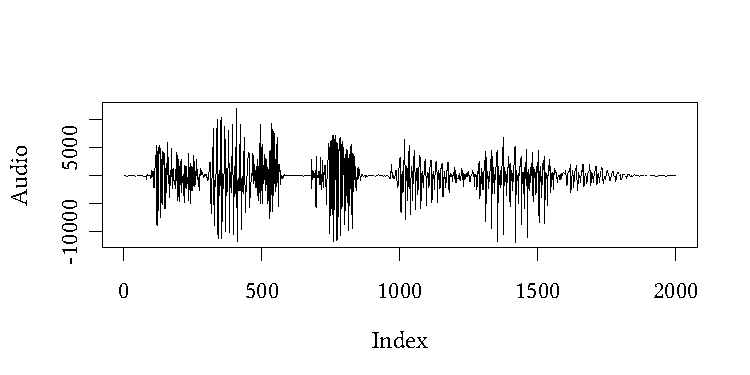
\includegraphics[width=\textwidth,height=.5\textwidth]{figure/chunk4} 

\end{knitrout}






\end{document}
